%%%%%%%%%%%%%%%%%%%%% chapter2.tex %%%%%%%%%%%%%%%%%%%%%%%%%%%%%%%%%
%
%  
%
% Use this file as a template for your own input.
%
%%%%%%%%%%%%%%%%%%%%%%%% Springer-Verlag %%%%%%%%%%%%%%%%%%%%%%%%%%
%\motto{Use the template \emph{chapter.tex} to style the various elements of your chapter content.}










\chapter{Constant Depth Circuit Lower Bounds}
\label{hastad} % Always give a unique label
% use \chaptermark{}
% to alter or adjust the chapter heading in the running head

%\section{Defining constant depth circuits}

Recall \Cref{def:boolean-circuit} of Boolean circuits.
We define the \emph{\textbf{depth}} of a Boolean circuit $C$ as 
the maximal length (i.e., number of edges) in a path from 
a leaf to the output node.

Here is an example of a circuit of depth 3:
\begin{figure}
    \centering
    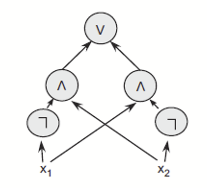
\includegraphics[width=0.2\linewidth]{images/depth_3_circuit.png}
    \label{xxx}
\end{figure}

\newcommand{\complexityclass}[1]{\sf{#1}}
\newcommand{\ACZ}{\ensuremath{\complexityclass{AC}^0}}


Recall that we are interested in the  study of the asymptotic size of circuit families, not a single circuit. That is, we want to consider how circuit size grows when the number of inputs $n$ grows. In this chapter we shall focus on circuit families $\{C_n\}_{n=1}^\infty$
whose number of inputs bits $n$ grows, their size $|C_n|$ grows polynomially while their depth is \emph{fixed} throughout the family, namly is a constant $c$ independent of $n$. 

%The class of Boolean functions computed by such circuit families is denoted $\ACZ$, and the class of such constant depth cir

%We can consider circuits of constant depth. This means that the depth of the circuit is \emph{independent of the number of inputs} $n$. In other words,  while $n$ the number of input gates can grow to infinity in the Boolean circuit family $\{C_n\}_{n=1}^\infty$, the depth of each circuit $C_n$ stays the same!


If the depth of the circuit is constant and the fan-in of gates is at most two, then the number of functions we can compute with such constant-depth circuits is constant. For example, the number of variables (appearing as leaves, i.e., input nodes) is constant that way, so for a large enough number of inputs $n$, we will not be able to compute functions that read all the $n$ inputs. This means that the model is \emph{not  complete}: for a constant $d$, a depth-$d$ circuit cannot compute all Boolean functions over $n$ inputs for every $n \in \mathbb{N}$.

To solve this problem and make the model of constant-depth
circuits meaningful we allow \textbf{\textit{unbounded} \emph{fan-in}} gates: unbounded fan-in AND gates: $\left(\varphi_1 \wedge \varphi_2 \wedge \ldots \wedge \varphi_\ell\right)$, and unbounded fan-in OR gates
$\left(\varphi_1\lor \cdots \lor \varphi_{\ell}\right)$, where the $\varphi_i$'s are circuits (of constant depth) by themselves, with possibly \emph{joint} nodes. 
\begin{figure}
    \centering
    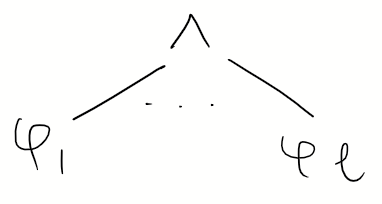
\includegraphics[width=0.2\linewidth]{images/AND.png}
    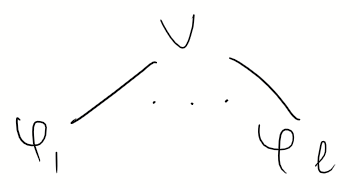
\includegraphics[width=0.25\linewidth]{images/OR.png}
    \caption{Illustration of unbounded fan-in AND and OR gates.}
\end{figure}



\newcommand{\depth}{\ensuremath{{\rm depth}}}

\begin{definition}[Depth-$d$ circuit family, constant-depth family]
\label{def:constant-depth-circuit}
A circuit family 
$\left\{\mathrm{C}_n\right\}_{n=1}^\infty$ with unbounded fan-in $\land,\lor$ gates and fan-in one negation gate is said to be of \emph{depth-$d$}, if the depth of $C_{n}$ is $d$, for all $n\in\N$. We denote by $\depth(C_n)$ the depth of the circuit $C_n$.
If $d$ is a constant (independent of $n$) we call $\left\{C_n\right\}_{n=1}^\infty$ a \emph{constant-depth family of circuits}.
\end{definition}

\textbf{Notation}: \ACZ\ denotes the complexity class 
consisting of all the functions $f:\{0,1\}^* \rightarrow\{0,1\}$ computable by  constant-depth circuit families  (equivalently, all decision problem decidable by \ACZ\ circuit families).

\para{Alternating Formulas}


We are going to use the following ``normal-form'' for constant-depth circuits. This is done for the sake of simplicity, and does not change the size of the circuits significantly, as we remark below.


A Boolean circuit is said to be an \emph{alternating  formula} if it is a formula (i.e., the underlying circuit graph is a tree), and every OR gate is followed by an AND gate followed by an OR gate, etc. Moreover, all negations in an alternating formula are pushed to the bottom of the circuit: that is, a negation node can only be connected to an input node (and that input node is not connected to any other node except a negation node). 
Here is an illustration:
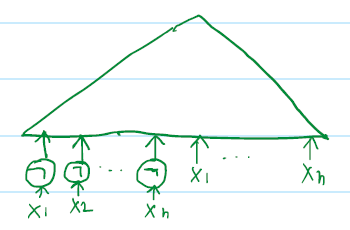
\includegraphics[width=0.3\textwidth]{image004.png}


% Always give a unique label
% and use \ref{<label>} for cross-references
% and \cite{<label>} for bibliographic references
% use \sectionmark{}
% to alter or adjust the section heading in the running head

For simplicity, we can assume that a constant-depth circuit has two types of inputs: every variables $x_i$ has a negative copy $\overline x_i$ (thus, getting rid of the need to specify a negation gate explicitly).  

Note that in an alternating formula every \emph{layer} (equivalently, \emph{level}) of the circuit, namely, nodes of a given depth $l$, are all of the same type: either all $\land$, all $\lor$ or all input variables (positive or negative).



We shall assume that all \ACZ\ circuits are alternating formulas:


\begin{tcolorbox}[colframe=white, colback=gray!11, boxrule=0mm, sharp corners]
 \textbf{Important:} From now on, when speaking about constant-depth circuits (i.e., \ACZ\ circuits), we assume by default the fan-in of $\lor, \land$ gates  is \emph{unbounded} ($\neg$ has fan-in one), and the circuits are \emph{alternating formulas}, and the \textbf{depth} is defined as maximal number of alternations between $\land$ and $\lor$ gates (or vice versa), namely the number of layers in the formula,  excluding the bottom layer which contains only the input variables (positive or negative).  
\end{tcolorbox}

\begin{exercise}
Show that every depth-$d$ circuit can be transformed into an alternating formula of depth-$O(d)$ circuit and with all negation gates on the leaves, with a polynomial size increase only.

\noindent---

\noindent{\small Hint: we can "unwind" the circuit into a formula (a tree; that is, if we used a subcircuit more than once [namely, it has out-degree more than 1], we copy this subcircuit for each such usage). Because the depth is constant this will increase the size of the circuit by at most a polynomial (exponential in a constant---i.e., polynomial). To make the formula alternating, first push all the negation to the bottom, using \emph{de Morgan rules}. And then, add dummy edges and gates to make every path from leaf to the output gate alternating between OR and AND. These all incur a polynomial increase in size.
}
\end{exercise}



\newcommand{\Parity}{\ensuremath{\operatorname{PARITY}}}

%\section{Lower Bounds Against Constant-Depth Circuits for PARITY}

\section{The PARITY Function}

The function PARITY determines the parity of the total number of ones in the input bits:

\begin{tcolorbox}[colframe=white, colback=gray!11, boxrule=0mm, sharp corners]
$
\Parity(x_1,\dots,x_n): =
\begin{cases} 
1 & \text{if the number of 1's in } (x_1, x_2, \dots, x_n) \text{ is odd}, \\
0 & \text{if the number of 1's in } (x_1, x_2, \dots, x_n) \text{ is even}.
\end{cases}
$
\end{tcolorbox}

Equivalently, $\Parity$ is defined as the XOR of the input bits, denoted $x_1\parity\cdots\parity x_n$. Another equivalent definition is using modulus: $x_1+\cdots+x_n = 1 \mod 2$.

We denote by $\Parity_n$ the \Parity\ function restricted to inputs of length precisely $n$.

The main result in this chapter is the following:


\begin{tcolorbox}[colframe=white, colback=blue!11, boxrule=0mm, sharp corners]
\begin{theorem}[\ACZ\ lower bound for \Parity]
\label{thm:ACZ-lower bound}
Every circuit family of depth-$d$ computing the $\Parity_n$ function requires size $2^{\Omega\left(n^{\nicefrac{1}{(d-1)}}\right)}$.
\end{theorem}
\end{tcolorbox}



Note: this means that if $d$ is constant, then the size lower bound is exponential: $2^{\Omega\left(n^{\nicefrac{1}{(d-1)}}\right)}=
2^{\Omega\left(n^k\right)}$, for some constant $0<k<1$.

The theorem is a consequence of the fact that every function in \ACZ\ can be reduced to a constant function by setting relatively few variables to constants.
The proof uses the Random Restriction Method described in the sequel.

\section{The Skeleton of the Lower Bound Argument}



\begin{tcolorbox}[colframe=white, colback=gray!5, boxrule=0mm, sharp corners]
\textbf{Upshot of argument}: The idea is to randomly restrict (assign) the variables of the circuit (of which we want to show it cannot compute \Parity). If the circuit is small, such a restriction collapses (gradually) the depth of the circuit to a depth-2 circuit. If the depth of the initial circuit was constant, this gradual step-by-step depth reduction needs to be done only for a constant many times. If we made random assignments (restrictions) only for a constant many times, we can rest assure that we have not assigned (i.e., fixed) too many variables. Hence, the function $\Parity$ under these restrictions still has a lot of free variables. But such $\Parity$ with sufficiently many free variables cannot have small depth 2 circuits (this we show by an auxiliary elementary argument).
\end{tcolorbox}

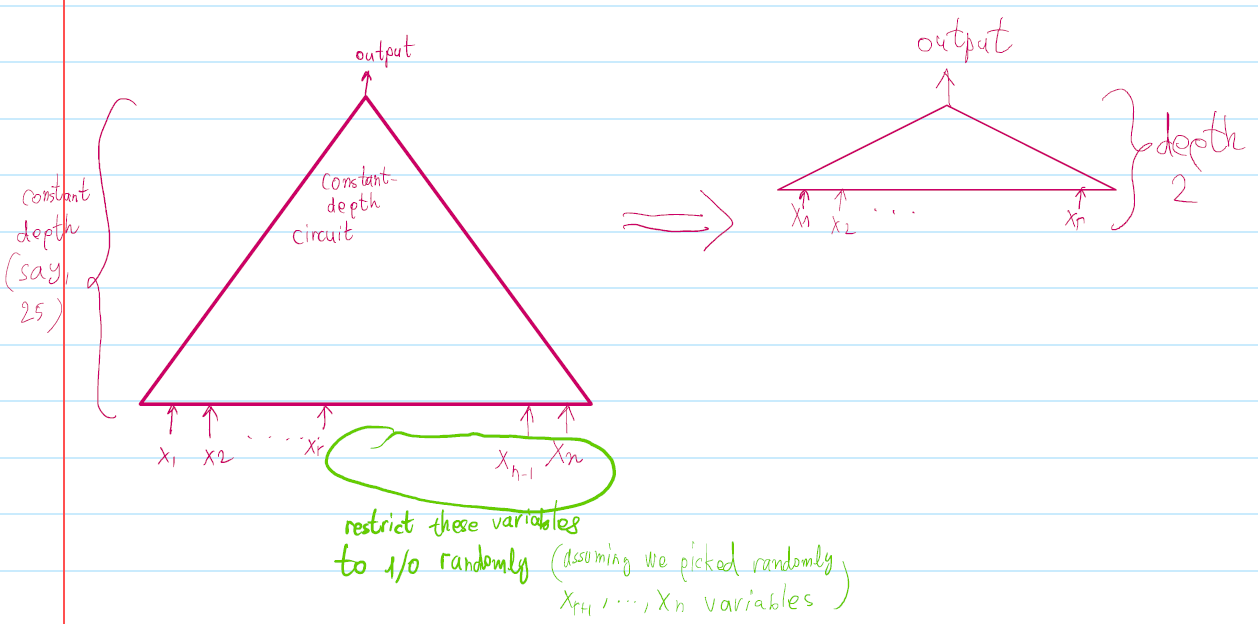
\includegraphics[width=0.9\textwidth]{image007.png}


\begin{note} Notice the similarity with the monotone circuit lower bound proof: we use structural induction on the circuit purported to correctly compute \Parity. \end{note}

\medskip
Here are the main steps of the argument with slightly more detail.

\para{Random Restriction Method: Structure of Argument}

\begin{enumerate}
\item By  way of contradiction, start with a purported small depth-$d$ circuit $C$ for $\Parity_n$.
We are going to assign to some of the input variables of the circuit $C$ (and hence, also to the function $\Parity_n$ it is supposed to compute), random 0,1 values. We show the result of these assignments leads to conflicting effects: with high probability, while the circuit restricted to these randomly chosen partial assignments becomes a circuit that computes a very simple function, the function $\Parity$ is still a rather complicated function to compute even after all these restriction.
\item Let $\overline x$ be $n$ variables $x_1,\dots,x_n$. Pick a random assignment $\rho_0: \overline x \rightarrow\{0,1, *\}^n$ with ``$x_i \rightarrow *$'' meaning that $x_i$ is \emph{un-assigned}, namely, stays a \emph{free} variable. We make sure that enough $x_i$'s stay  free, as this is crucial to get our contradiction.
\label{it:two-165}

\item Depth Reduction Step: 
%\item   $f$ is resilient in the sense that $f\rst\rho
%%\not\equiv 0$;

\begin{enumerate}
\item 
If $C$ is a small circuit then the \emph{function} computed by $C\rst\rho_0$, namely the restriction of $C$ to the assignment $\rho_0$, has a depth  $d-1$ circuit of small size. 

\item
Sequentially we assign new further random restrictions $\rho_1,\dots,\rho_{d-3}$
 (extending $\rho_0$) so that we reduce the depth of $C$ by 1 each time, until the depth is 2.
\end{enumerate}

\item 
At this point, we end up with a circuit $C^{\prime}$ of depth 2, namely a $k$-DNF or a $k$-CNF, for some small $k$ that computes the function 
$\Parity_n\rst\rho_0\rho_2\ldots\rho_{d-3}$.

\item
We now use an auxiliary statement to reach a contradiction: since we made sure that each assignment $\rho_i$ leaves enough variables free, 
$\Parity_n\rst_{\rho_0\rho_2\ldots\rho_{d-3}}$ is the PARITY function on $k'$ variables, i.e., $\Parity_{k'}$. But this is still a relatively "complex" function:
in particular, it is a very simple argument to show that there are no $k$-CNF formulas for $\Parity_{k'}$, whenever $k'>k$, which will conclude the argument.
\label{it:final-step:269}
\end{enumerate}


\begin{figure}
    \centering
    \includegraphics[width=0.4\textwidth]{images/hastad-sitter-600.jpg}
    \caption{Johan H\aa stad}
\end{figure}


\subsection{Depth Reduction Step: the Switching Lemma}

We shall use the following notation.
\begin{itemize}
    \item \textit{Boolean (propositional) variables:} \(x_1, x_2, \ldots \).
    \item \textit{Literal:} \(x_i\) or \(\neg x_i\) (i.e., a variables or its negation).\\
    A negation of a variable  \(x_i\) is written as eiter \(\neg x_i\), or $\overline {x_i}$.
    \item \textit{Clause:} A disjunction of literals.\\
    Example: \((x_1 \lor \neg x_2 \lor x_3)\)
    \item \textit{CNF:} Conjunctive Normal Form formula, namely a conjunction  of clauses.\\
    Example: \((x_1 \lor \neg x_2 \lor x_3) \land (x_1 \lor x_4 \lor x_5) \land (x_2 \lor \neg x_7 \lor \neg x_{20} \lor \neg x_{102})\)
    \item \textit{DNF:} Disjunction Normal Form formulas, namely a disjuncion of ANDs of literals (an AND of literals is sometimes called \emph{a term}.\\
    Example: \((x_1 \land x_4 \land x_7) \lor (x_8 \land \neg x_9 \land x_{10}) \lor (x_3 \lor \neg x_2)\)
    \item \textit{$t$-clause:} A clause with at most \(t\) literals.\\
    Example: 3-clause: \((x_1 \lor \neg x_2 \lor x_7)\)
    \item \textit{$t$-CNF:} A CNF with all clauses being \(t\)-clauses.
    \item \textit{$s$-DNF:} A DNF with all terms  having at most \(s\) literals.
\end{itemize}


The below figure illustrates a single Depth Reduction Step. Such a step is also called  ``Switching'', as it switches a $t$-CNF into an $s$-CNF, or vice versa.

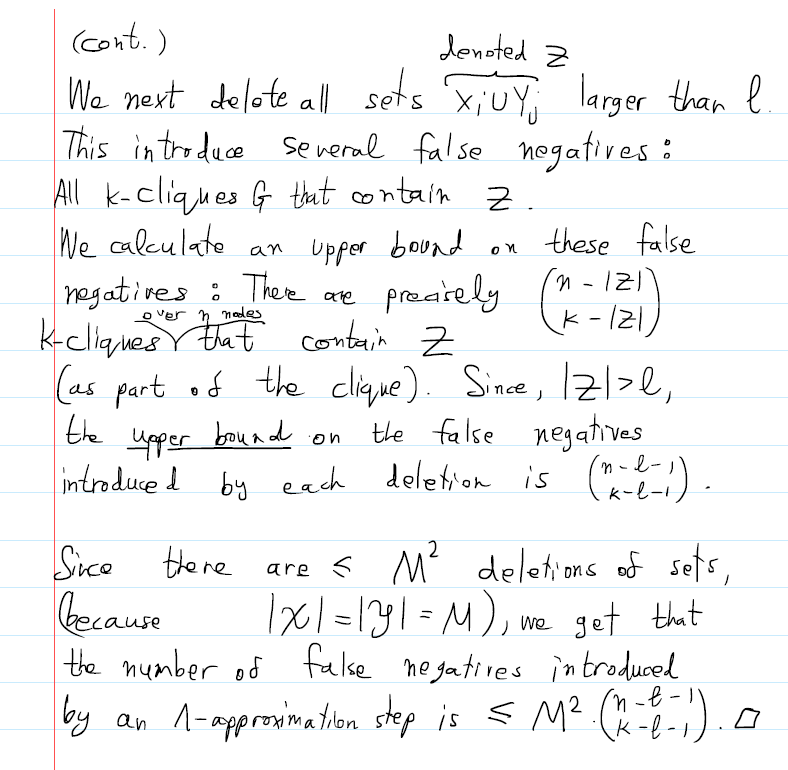
\includegraphics[width=0.7\textwidth]{image008.png}

\begin{note} We can always turn a $t$-CNF into an $s$-DNF for some \textit{big} $s$ (by distributing out \(\lor, \land\) using de Morgan's rules).
But then we've not maintained the invariant that the bottom level has fan-in \(\leq s\) (namely, \(s\) is small enough).
In other words, we will end up with a depth-2 circuit, but of huge size computing \(f\rst_\rho\). This will not give us a contradiction since every function is computable by an exponential-size circuit.
\end{note}

\para{Examples of Assignments and their Consequences}
\emph{How can we  turn a $t$-CNF into an $s$-DNF while keeping $s$ small}?
We can turn the $t$-CNF to a (general) DNF using de Morgan rules (just distribute $\wedge$ over $\vee$), for example
\[
(x_1 \vee \bar{x}_2) \wedge (x_3 \vee \bar{x}_4) \equiv (x_1 \wedge x_3) \vee (x_1 \wedge \bar{x}_4) \vee (\bar{x}_2 \wedge x_3) \vee (\bar{x}_2 \wedge \bar{x}_4),
\]

and then try to \emph{eliminate literals} in big ANDs by using assignments to the literals in those terms. This may reduce indeed the size of terms, and if we do this enough we may be able to reduce all the terms that are wider than $s$.
 
 
Consider the following DNF:
\[
(x_1 \wedge x_2 \wedge \bar{x}_3 \wedge \bar{x}_5 \wedge \bar{x}_8) \vee ( \dots \wedge \bar{x}_9 \wedge \dots)\lor\dots.
\] We can assign $1$ to $x_2$ and $1$ to $x_9$. In the first conjunct (i.e., the first AND or term) it results in the \emph{deletion of $x_2$}, while in the second conjunct, it results in \emph{deletion of the whole conjunct}:

Assigning $1$ to $x_2$:
\[
(x_1 \wedge x_3 \wedge \bar{x}_5 \wedge \bar{x}_8) \vee ( \dots \wedge \bar{x}_9 \wedge \dots )
\]
Assigning $1$ to $x_9$:
\[
(x_1 \wedge x_3 \wedge \bar{x}_5 \wedge \bar{x}_8) \vee \underbrace{( \dots\wedge 0 \wedge \dots)}_{\text{false}} 
\]





\begin{note}\
\begin{enumerate}
    \item Literal $l_j \from 0$ (i.e., assigning $0$ to literal $l_j$)
    \[
        (l_j \wedge D) \equiv \text{false}.
    \]
    So the whole AND disappears.
    
    \item Literal $l_j \from 1$:
    \[
        (l_j \wedge D) \equiv D.
    \]
    So we reduced the size of the AND by $1$.
\end{enumerate}
\end{note}

But how can we choose the assignment of $0$ and $1$'s to variables that guarantees eliminating all the large conjuncts, without fixing all the variables in the DNF formula (recall that by \Cref{it:two-165} above we need to keep sufficiently many variables $x_i$ free)?
The idea is to use the \emph{probabilistic method}: choosing a \emph{random} $g: \overline x \to \{0,1, *\}^n$ will lead with \textbf{positive} probability to an assignment that eliminates \emph{all} large conjuncts, while leaving enough variables free. When an event occurs with a positive probability, in this case the event of choosing an assignments with the desired properties, it means that there \textbf{exists} at least one such assignment. This will be enough for our purpose: the existence of such an assignment is sufficient to conclude our proof, because our argument hinges on a proof by contradiction: if there exists a small constant-depth circuit for PARITY, then there \emph{exists} also a desired assignment (formally, a sequence of assignments) that will yield our contradiction as in \Cref{it:final-step:269}.

\para{Switching via Random Restrictions}

\textbf{Notation:} 
\begin{enumerate}
\item 
 A \textit{restriction} $\rho$ for $l$ variables in $\bar{x}$ is a function $\rho: \bar{x} \to \{0,1, *\}$, assigning either 0, 1 values to the variables or leaving them free, namely $\rho(x_i) = *$ means that $x_i$ is \textit{unassigned} (or ``free'') according to $\rho$.

 
\item For a function $f: \{0,1\}^n \to \{0,1\}$ and a   restriction $\rho: \bar{x} \to \{0,1, *\}$, we write $f\upharpoonright \rho$ to denote the function $f$ where the variables are set according to $\rho$.
%and $\rho(x_i)$ means $x_i$ is \textit{left unassigned}.

If we then apply another restriction $\tau$ to the variables in $f\upharpoonright \rho$, we 
write $f\upharpoonright_{\rho\tau}$ to denote $(f\upharpoonright \rho)\upharpoonright \tau$. In other words,
\[
f\upharpoonright_{\rho\tau} = f\upharpoonright_{\rho \cup \tau}
\]
where $\rho \cup \tau$ is the union of two functions.
\end{enumerate}



\begin{tcolorbox}[colframe=white, colback=green!6, boxrule=0mm, sharp corners]
\begin{definition}
[Random Restriction]
 Let $0< p<1$.
Let $\cR$ be a distribution on partial restrictions $\rho$ to the variables $\overline{x}$ with $|\overline{x}|=n$ , as follows.
$$
\begin{aligned}
& ~~~~~~~~~~~ \quad \operatorname{Pr}\left[\rho\left(x_i\right)=*\right]=p \\
& \operatorname{Pr}\left[\rho\left(x_i\right)=0\right]=\operatorname{Pr}\left[\rho\left(x_i\right)=1\right]=\frac{1-p}{2}.
\end{aligned}
$$
\end{definition}
\end{tcolorbox}
In other words, we pick randomly and independently for each variable $x_i$ with $i\in[n]$, either to leave it free with probability $p$, or to fix it to 1 or 0 with equal probability $(1-p)/2$.


\begin{tcolorbox}[colframe=white, colback=blue!5, boxrule=0mm, sharp corners]
\begin{theorem}[Switching Lemma]
For every positive integers $r$ and $k$ and $n$, if a Boolean function $f$ with $n$ variables is computable by an $r$-DNF and $\rho$ is a random restriction as above with $0<p \leq \frac{1}{9}$, then with probability at most $(9pr)^s$, $f\!\rst_\rho$ \emph{cannot} be computable by as an $s$-CNF.
\end{theorem}
\end{tcolorbox}

The Switching Lemma thus shows that the ``bad'' event of a function computed by an $r$-DNF formula not being able to switch, under  a random restriction,  to a function that can be computed by an $s$-CNF, is small. This would mean that with high enough probability the ``good'' event happens: a random assignment switches an $r$-DNF to an $s$-CNF.
In practice, we usually need to have the probability of the bad event to be \emph{really} small, in this case  exponentially small, so that the probability that \emph{none} of a collection of bad events happens in the random experiment is small (using the union bound), and specifically smaller than 1, to be able to claim there exists an object with the required properties (in our case, an assignment that would switch exponentially many $r$-DNFs).  

However, we note that this probabilistic argument via the union bound  is  \emph{not} sufficient to conclude the argument. We shall also need to make sure that such a ``good'' random assignment  \emph{leaves many variables free}. For this purpose, we will use a common tool in probabilistic analysis and concrete complexity: \emph{concentration bounds} (in our case it will be the Chernoff Bound). We  explain this point in the the next section when proving the lower bound.


\begin{exercise} Show that by applying the Switching Lemma to the function $\neg f$ we can get the same result with the terms ``DNF'' and ``CNF'' interchanged. Namely, the probability that an $r$-CNF does not switches to an $s$-DNF is at most $(9pr)^s$.
\end{exercise}

\section{Proof that PARITY does not have small circuits, using the Switching Lemma}

Recall that we want to prove \Cref{thm:ACZ-lower bound}  stating that every circuit family of depth-$d$ computing the PARITY function requires size $2^{\Omega\left(n^{\nicefrac{1}{d-1}}\right)}$.

So, suppose  that $C$ is a depth-$d$ alternating formula circuit of size $s$ computing $\Parity_n$. We are going to show that $s= 2^{\Omega\left(n^{\nicefrac{1}{d-1}}\right)}$, since assuming otherwise would lead to a contradiction.


Recall that we assume that $C$ is an alternating formula, with $d$ layers, where in each layer all gates are either $\land$ or $\lor$.  The proof proceeds by first a ``preprocessing step'' in which we use the Switching Lemma to decrease the fan-in of the \emph{bottom} layer gates, followed by   $d-2$ depth reduction steps using the Switching Lemma in which we gradually reduce the depth of the circuit, from bottom to top, by one depth, until we reach a depth-$2$ circuit.
After this, we can conclude the theorem: if the circuit was too small, we end up with a $k$-CNF (or $k$-DNF) computing \Parity\ over more than $k$ variables which is easyly shown to be impossible.




% Enable watermark from this point onward
%\SetWatermarkText{DRAFT}



\para{Decreasing Bottom Layer Fan-in}

This step is needed in order to optimise the lower bound, namely to reach the tight lower bound of $2^{\Omega(n^{1/d-1})}$. \% we may explain this point later.

Consider the bottom two layers of the given constant-depth circuit. We assumed that the layers alternate between $\land$ and $\lor$, thus the depth-2 sub-formulas  at these bottom two layers are all either DNFs or CNFs. Let us assume  without loss of generality  that they are all CNFs. The bottom fan-in of these CNFs may be large, namely, it may be $\ell$-CNFs for a large $\ell$. 
Since  $\ell$ may be  very large, using the Switching Lemma to turn this $\ell$-CNF to an $s$-DNF will be too expensive, in the sense that applying the Switching Lemma with this $\ell$ would give us probability of $\leq (9p\ell)^s$, but with \emph{large} $\ell$, which later would mean we get a weaker lower bound (e.g., we sould get a lower bound of $2^{\Omega(n^{\frac{1}{d}})}$, which is weaker, namely smaller, than our lower bound of $2^{\Omega(n^{\frac{1}{d-1}})}$).
\textcolor[rgb]{0.815686,0.815686,0.815686}{\% This is caused by a weaker union bound computation (we explain this after we finish the proof).}



For this reason, we shall reduce the fan-in of the bottom layer (i.e., layer 1) directly using the Switching Lemma (while maintaining a lower probability of failure).

\begin{claim}\label{cla:}
An $\ell$-CNF does not turn into a $k$-CNF under a random restriction $\rho$ with probability $\leq (9p_0)^k$, for $p_0$ the probability a variable is free in the random restriction $\rho$. Specifically, when $k = 2 \cdot \log S$, if we choose $p_0 = \frac{1}{18}$, the probability of failure is at most $ \frac{1}{S^2}$.
\end{claim}

\begin{proof}[Claim]
The below figure illustrates  the simple argument:

\begin{center}
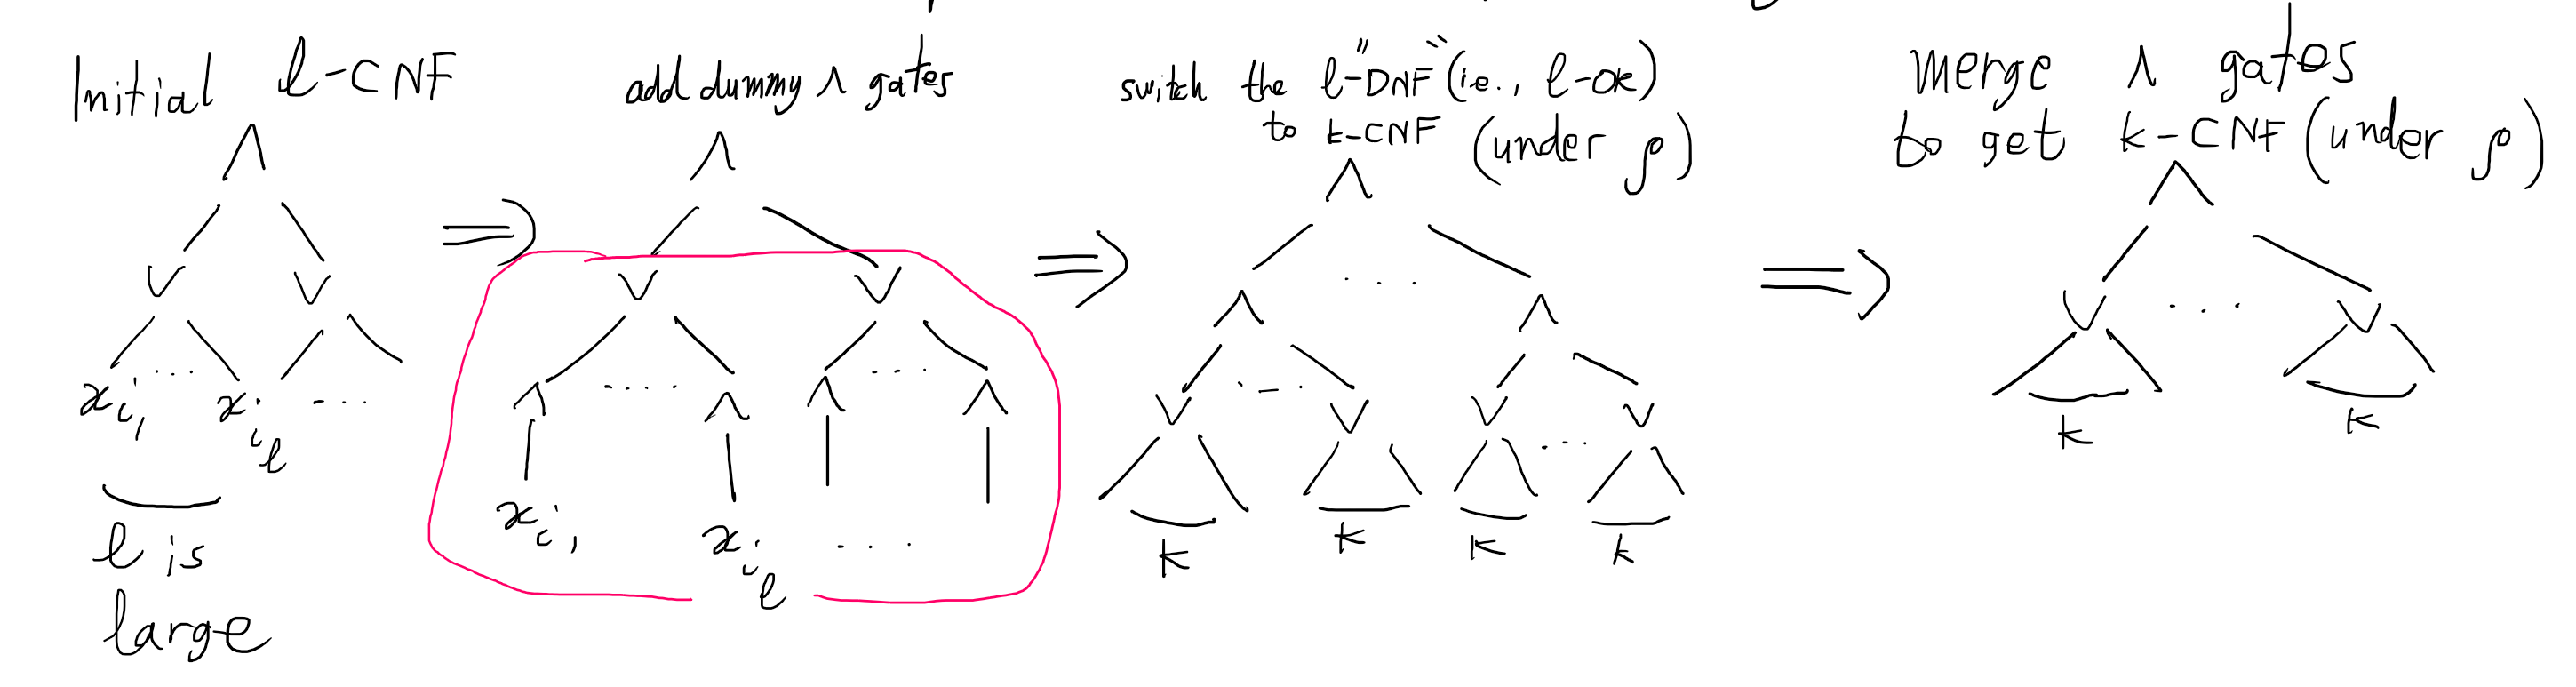
\includegraphics[width=\textwidth]{images/bottom-layer-switch.png}
\end{center}


In particular, we switch the lower 1-DNFs (\emph{in red}) into $k$-CNF with a random restriction, so by the Switching Lemma, the probability the switching fails is 
\[
\leq (9 \cd p_0 \cd1)^k = (9 \cdot \frac{1}{18})^{2 \cdot \log S} = \frac{1}{2^{2 \cd\log S}} = \frac{1}{S^2}.
\]
\
\end{proof}

By this claim, and using the union bound, the probability that at least one $\ell$-CNF in layer 2 does not switch is at most $ S\cd 1/S^2 = 1/S$.



\para{Repeated Depth Reduction Steps}
We now start from a circuit $C{\rst}_{\rho_1}$ with $k$-CNF at the bottom, for $k = 2 \log S$.
We go by induction on depth, to prove the following.


\begin{tcolorbox}[colframe=white, colback=red!11, boxrule=0mm, sharp corners]
\begin{lemma}[Induction Statement]\label{lem:induction-switch}
Let $C$ be a depth at least $d$ circuit of size $S$ 
with layer-1 (bottom) gates all of fan-in  $ \leq k=2 \log S$ (either  $\land$ or $\lor$),
with $n$ input variables  
$\overline x$ (with positive and negative copies). Assume that the gates in layer $d$ are all $\land$ gates (resp., $\lor$ gates). 
Then, there exists a restriction $\rho: \overline {x} \rightarrow\{0,1, *\} $ with at least  $\frac{p^{d-2} \cdot n}{2^{d-2}} $ free variables, where $ p=\frac{1}{36 \cdot \log S}$, such that  
the function computed by $g{\rst}_{\rho}$ for every $\land$ (resp. $\lor$) gate in layer $d$ is computable by a $k$-DNF (resp., a $k$-CNF). 
\end{lemma} 
\end{tcolorbox}

\begin{proof}[\Cref{lem:induction-switch}]
We prove it for the case $\land$ in layer $d$. The $\lor$ case is similar.  

\Base $d = 2$. Since the bottom layer is assumed to be of fan-in $\leq k$,  
this case holds immediately.  

\Induction   
We assume the induction statement holds for layer $d-1$, and prove it for $d$. The following figure illustrates the argument. 




\begin{figure}[H]\label{fig:depth-reduction-use}
    \begin{center}
    \includegraphics[width=\textwidth]{switchinginduc.png}
    \end{center}
\end{figure}


\textit{The setup of the induction step}: In (\textbf{1}) in the figure,  we have (by induction hypothesis) a depiction of part of the circuit $C$, showing a single $\land$ gate in layer $d$ (there  may be other $\land$ gates in this layer, and there may be other gates above it in layers higher than $d$). 
In (\textbf{2}) we see the $\land$ gate in layer $d$ under the restriction $\rho'$, i.e., $C\rst_{\rho'}$, with $\rho'$ having $\geq \frac{p_0^{d-3} \cdot n}{2^{d-3}}$ free variables. Hence, its children, which are $\lor$ gates, have turned under $\rho'$ to  $k$-CNFs.
 (\textbf{3}) simply merged the $\land$ gate in layer $d$ to its children in layer $d-1$, all of which turned to $\land$ gates themselves. 
Our goal is to get to circuit (\textbf{4}), by applying the Switching Lemma with a random restriction $\rho''$ and then compute an upper bound on the probability that such a switch to $k$-DNF occurs for \emph{all} the gates in layer $d$. We explain this now.


\smallskip 

% \begin{theorem}[Switching Lemma]
% For every positive integer $r$ and $k$ and $n$,  
% if a Boolean function $f$ with $n$ variables is computable by an $r$-DNF  
% and $\rho$ is a random restriction as above with $0 < p \leq \frac{1}{9}$,  
% then with probability at most $(9pr)^k$, $f_{|\rho}$ cannot be computable  
% by an $s$-CNF.
%\end{theorem}


Using the Switching Lemma with the parameters \( r = s = k = 2 \log S \), with probability \( \leq (9pk)^k \), a \emph{single} $k$-CNF in layer \( d \) does not switch to a $k$-DNF.
By the union bound, with probability \( \leq S\cd(9pk)^k \) the bad event that \emph{at least one} $k$-CNF in layer \( d \) does \emph{not} switch to a $k$-DNF occurs.
We now use another bound to estimate the probability of the event that a random restriction has too few free variables. The tool we use is the Chernoff bound.


\begin{tcolorbox}[colframe=white, colback=gray!11, boxrule=0mm, sharp corners]
\textbf{Chernoff Concentration Bound}.
Random variables and expectations: A random variable \( X \) is a mapping from the sample probability space of elementary outcomes to the real line, \( X: \Omega \to \mathbb{R} \). For example, consider a random variable with \( X_i = 1 \) if \( E_i \) occurs, and \( 0 \) otherwise. (For example, a random event is flipped as ``heads'') The indicator variable \( X \) taking values in \( [0, 1] \), with \( X_i = 1 \) if \( E_i \) happened, \( 0 \) otherwise.

If a random variable \( X \) takes its values from a set \( A \), we define the expectation of \( X \) as follows:
\[
\mathbb{E}[X] = \sum_a Pr[X = a]a
\]

Linearity of expectation: For random variables \( X_1, X_2, ..., X_n \), (not necessarily independent), we have:
\[
\mathbb{E} \left[ \sum_{i=1}^{n} X_i \right] = \sum_{i=1}^{n} \mathbb{E}[X_i]
\]

Concentration around the expectation: 
For a random variable \( X = \sum^n_{i=1} X_i \), that is a sum of independent random variables (say each \( X_i \) takes values in \( \{0, 1\} \)), a much stronger bound is given by the Chernoff inequality. In particular, it says that the probability that this \( X \) is at least twice the expectation is inversely-exponentially small in the expectation.

\begin{theorem}[Chernoff\,bound] Let \( X_1, X_2, ..., X_n \) be independent identically distributed random variables such that \( Pr[X_i = 1] = p \) and \( Pr[X_i = 0] = 1 - p \), for some \( 0 \leq p \leq 1 \).
Consider the new random variable \( X = \sum X_i \), with expectation \( \mu = pn \). Then, for any \( 0 < \delta < 1 \),
\[
Pr[|X - p| > \delta p] \leq 2 e^{- \frac{\delta^2 \mu}{3}}.
\]
\end{theorem}
\end{tcolorbox}



\
\

We apply Chernoff bound to our case as follows.
Every single variable \( x_i \) has a probability \( p \) to stay free under our new restriction  \( \rho'' \).
Hence, the expected number $\mu$ of free variables is \( pN \), where $N$ is the number of (free) variables in $C\rst_{\rho'}$ which is $\ge \frac{p^{d-3} \cdot n}{2^{d-3}}$ by induction hypothesis. Hence, the expected number of free variables is $\mu\ge pN= \frac{p^{d-2} \cdot n}{2^{d-3}}$. 
(Since the event that a variable stays free under \( \rho'' \) is independent from the events that other variables stay free, the expected value is achieved with high probability by the Chernoff bound.)
 In other words, the bad event that the number of free variables are less than half of the expected value $\mu$ is at most $
2e^{-\delta^2 \cdot \frac{\mu}{3}}$, with $\delta = \frac{1}{2}$ and  $\mu = \frac{p^{d-3} \cdot n}{2^{d-2}}.$

The following is thus the upper bound on the probability that at least one bad event happened (using the union bound): 
\begin{equation}\label{eq:487:28}
 S(9pk)^k + 2e^{-\delta^2 \cdot \frac{\mu}{3}}, \quad with \quad \delta = \frac{1}{2} \quad \text{and} \quad \mu = \frac{p^{d-3} \cdot n}{2^{d-3}},
\end{equation}
where the left most term is by a union bound on all gates, and the rightmost term is the bad event estimated by the  Chernoff bound.\footnote{%
Note that we have used the union bound on the following bad events, given a random pick of a single assignment $\rho$: $S$ many potential bad events that a gate in layer $d$ does not switch, together with a single event that the number of free variables in $\rho$ falls below half the expected number of free variables.
}


All that is left is to make some computations to get a lower bound on the parameter $S$. 

\Cref{eq:487:28} is equivalent to 
\[
S \left( 9 \cdot \frac{1}{36 \cdot \log s} \cdot 2 \log s \right)^{2 \log s} + 
2 e^{-\frac{\left(\frac{1}{36 \cdot \log S }\right)^{d-3} \cdot n}{2^{d-1} \cdot 3}}.
\]


Let us denote the right summand above by $B$. 
We get:
$$
=S \cdot\left(\frac{18}{36}\right)^{2 \cdot \log S}+B =S \cdot \frac{1}{S^2}+B =
\frac{1}{S}+
\underbrace{
    e^{
        \frac{2}{
        \frac{n}{{(36 \cdot \log S)^{d-3} \cdot 2^{d-1} \cdot 3}}}}
}_B
$$

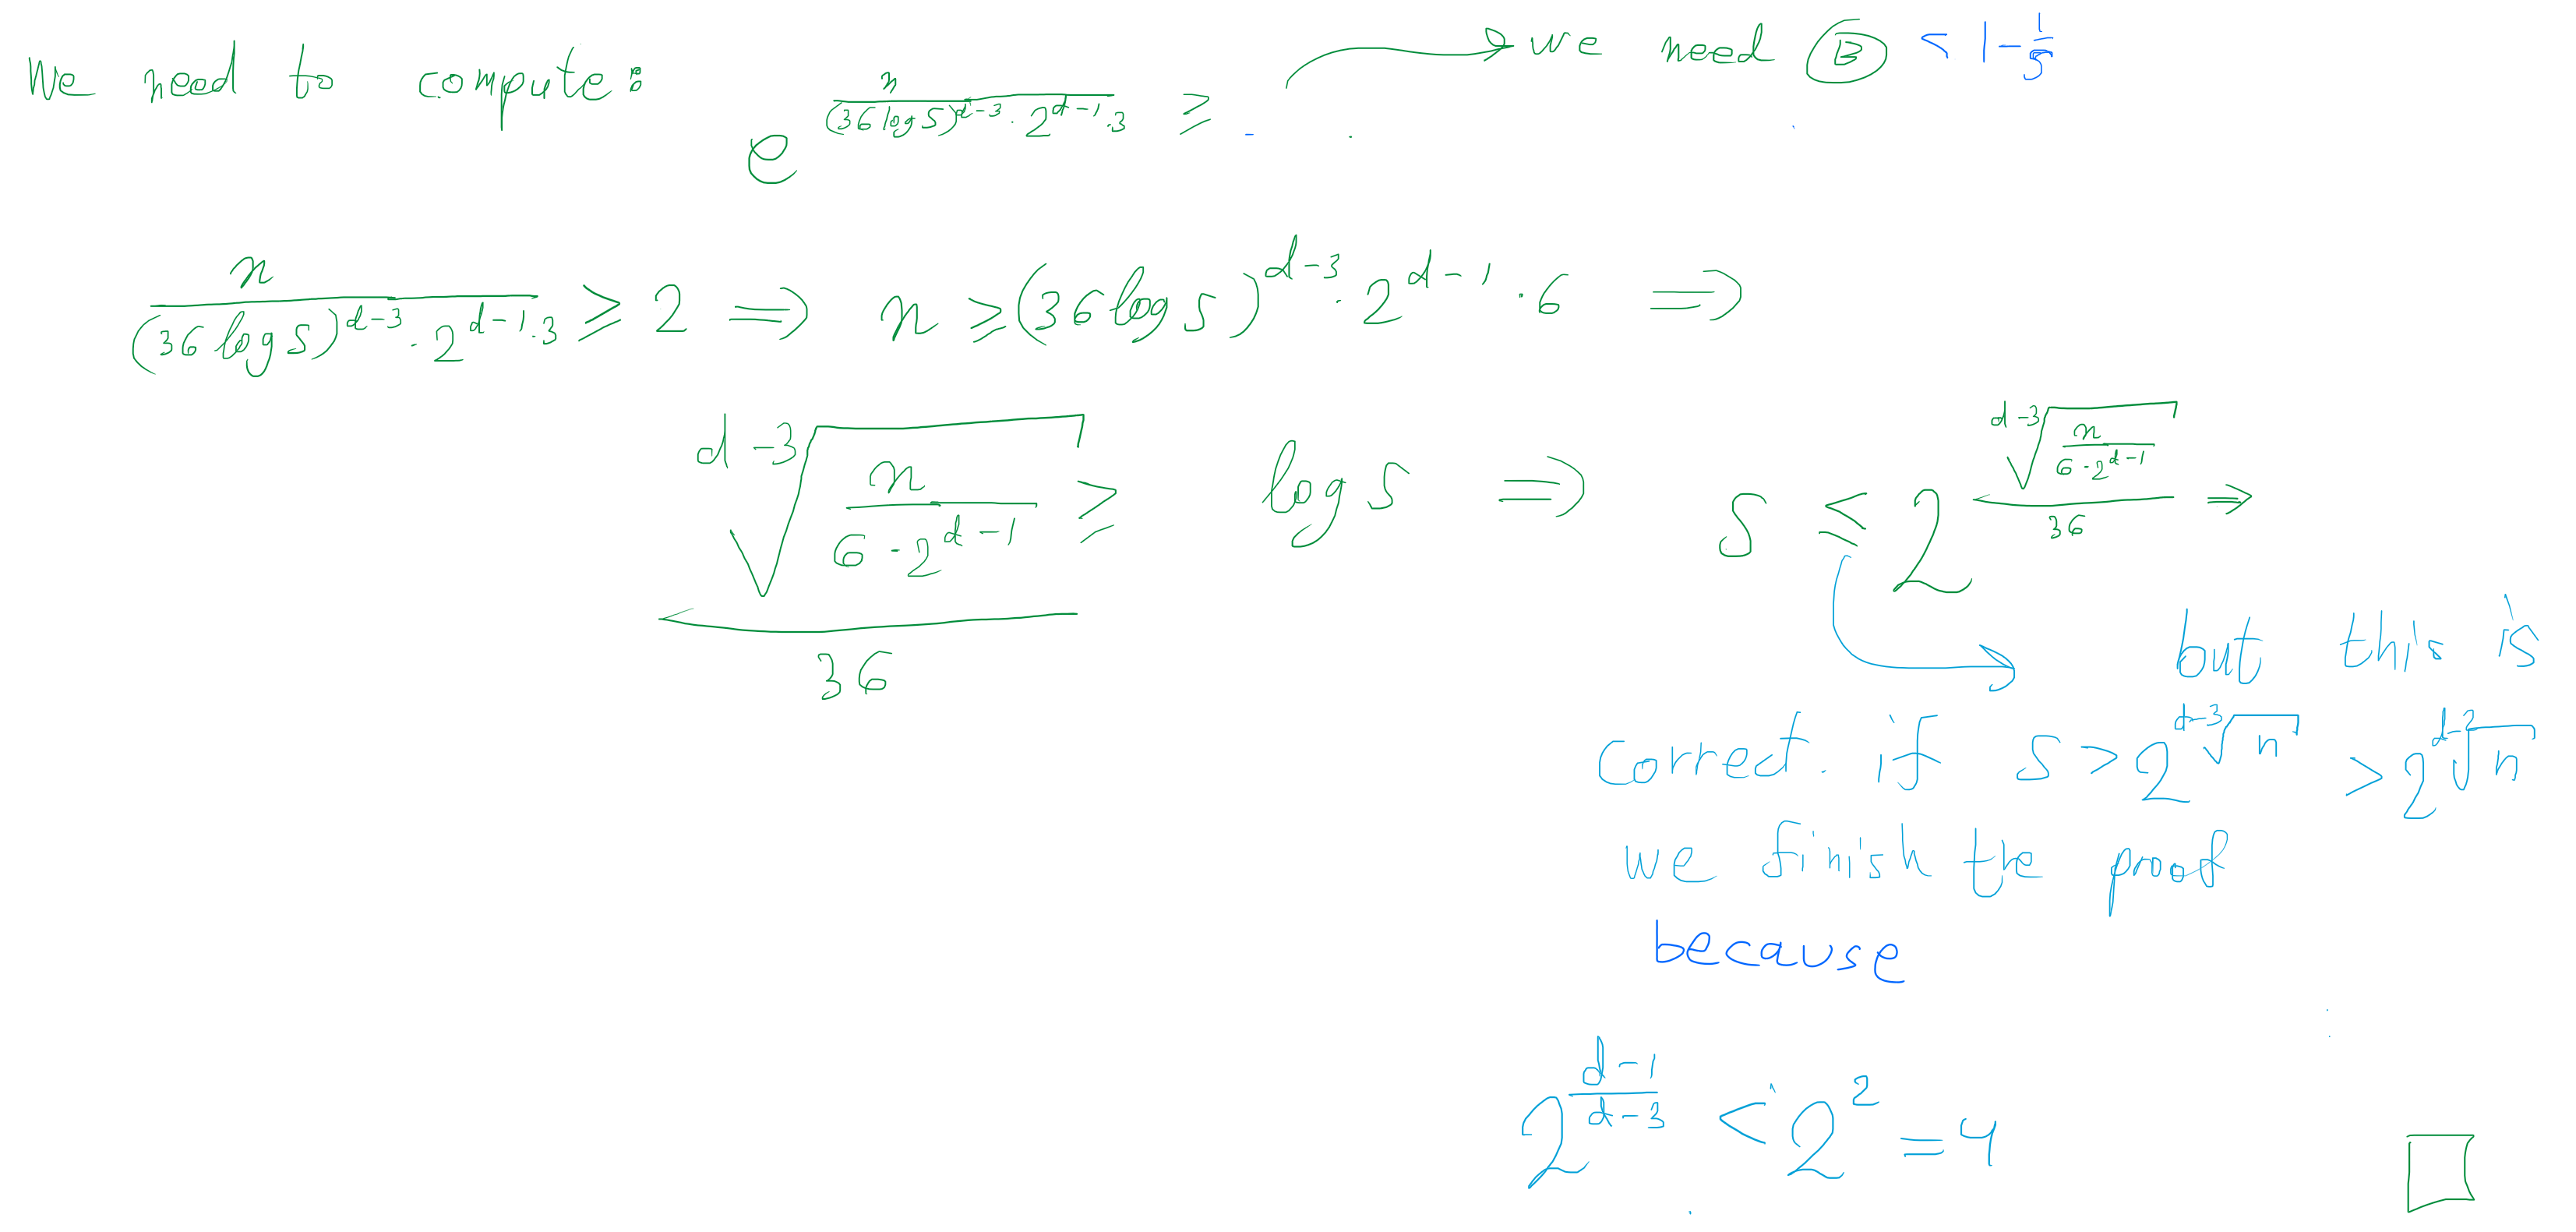
\includegraphics[width=\textwidth]{image010.png}

(Note: 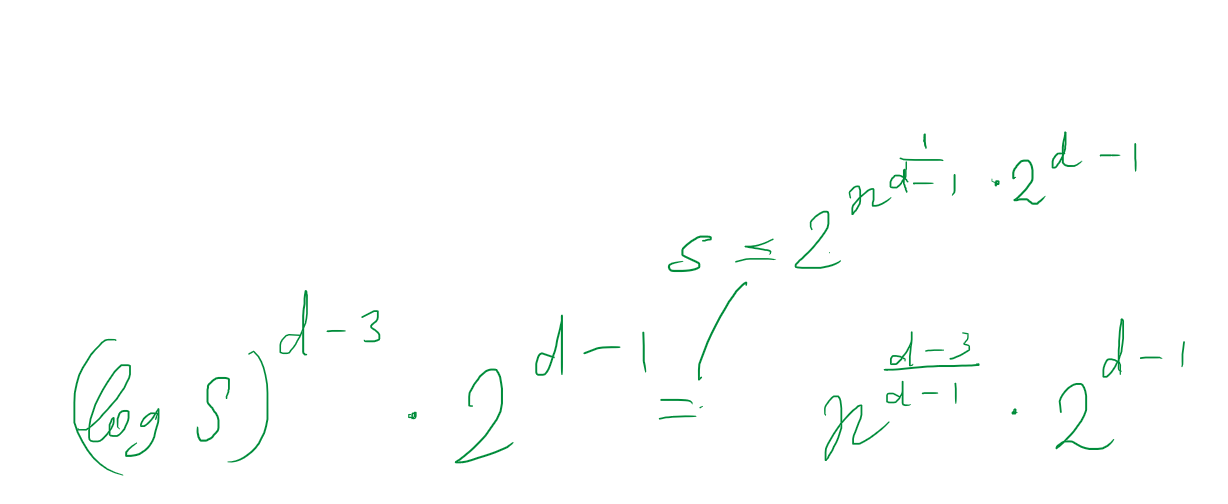
\includegraphics[width=0.3\textwidth]{image011.png})
\mbox{}
\end{proof} % Induction step of Switching


\para{Concluding the proof}
Using the Induction Statement together with the Bottom Switching Step,
we can now conclude the proof of the lower bound.
Given a circuit of depth $d$ with $n$ variables,
we first apply the Bottom Layer Switching (with sufficiently high probability using Chernoff's bound, the number of free variables after this step
are at least $(1/36)\cd n$; we skip this computation).

Then, we have a circuit $C$ of depth-$d$ with layer 2 consisting of  $k$-CNF gates. We  then apply the Induction Statement. We reach a circuit $C \rst_\rho$ of depth-2, namely a $k$-CNF (or $k$-DNF) with
$\rho: \bar{x} \rightarrow\{0,1, *\}$ being a restriction
with $\geq \frac{p^{d-2} \cdot n}{2^{d-2}}$ free variables and $p=\frac{1}{36 \cdot \log S}$, such that the function computed by $g\rst_\rho$ for every $\land$ gate $g$ in layer $d$ (resp., $\lor$ gate) can be computed by a $k$-DNF, with $k=2 \log S$ (resp. a $k$-CNF).
And specifically, when $d$ is the depth of $C$, we know that $C\rst_\rho$ as a whole is computed by a $k$-CNF (in this case $d$ is a layer with a single gate). 


But now we get a contradiction if \( k \) is less than the number of free variables, which is 
\[
\frac{p^{d-2} \cdot n}{2^{d-2}}.
\]
This is because every \( k \)-CNF can be made the  constant function 0 with \( k \) assignments of 0/1 values to its variables: Pick one \( k \)-clause, e.g.,
\[
x_1 \lor \overline{x_2} \lor x_3 \lor \overline{x_4},
\]
assign the literals in the clause all zero: 
\[
x_1 = 0, \ x_2 = 1, \ x_3 = 0, \ x_4 = 1.
\]
However, Parity for \( r > k \) cannot be made a constant function without assigning all its \( r \) variables. Hence, when the number of free variables
\[
\frac{p^{d-2} \cdot n}{2^{d-2}} > k = 2 \log S,
\]
we get  a contradiction.
In other words, we have:
\[
2 \log S \geq \frac{p^{d-2} \cdot n}{2^{d-2}}.
\]
We now compute to find out what is the lower bound for $S$:
\begin{align*}
    2 \log S &> \frac{p^{d-2} \cdot n}{2^{d-2}} 
 = \frac{\left(\frac{1}{36 \log S}\right)^{d-2} \cdot n}{2^{d-2}} 
    & = \left(\frac{1}{\log S}\right)^{d-2} \cdot n \cdot \left(\frac{1}{72}\right)^{d-2}.
\end{align*}
Hence, 
\begin{align*}
    \left(\log S\right)^{d-1} &> \frac{1}{2} \left(\frac{1}{72}\right)^{d-2} \cdot n \implies \\
    \log S &> \frac{1}{2} \left(\frac{1}{72}\right)^{\frac{d-2}{d-1}} \cdot n^{\frac{1}{d-1}} \implies \\
    \log S &= \Omega \left(n^{\frac{1}{d-1}}\right) \implies 
    S= 2^{\Omega ({\sqrt[d-1]{n}})}.
\end{align*}

 Concluding the proof. 
 \hfill $\Box$

% 
% \textbf{And specifically}, when $d$ is the depth of $C$, we know that $C_{\beta}$ as a whole is computed by a k-CNF.
% 
% But now we get a contradiction if $k$ is less than the number of free variables, which is:
% 
% $$ k \geq \frac{p^2 - n}{2} $$
% 
% This is because every k-CNF can be made a constant function (1) with $k$ assignments of 0/1 values to its variables:
% pick one clause, i.e., $x_1 \vee \bar{x_2} \vee x_3 \vee \bar{x_4}$,
% assign the literals in the clause all zero: $x_1 = 0, x_2 = 1, x_3 = 0, x_4 = 1$.
% 
% However, Parity for $k \geq k$ cannot be made a constant function without assigning all its variables.
% Hence, when the number of free variables:
% 
% $$ \frac{p^2 - n}{2} \geq k = 2 \log s $$
% 
% we get a contradiction.
% 
% In other words, we have:
% 
% $$ \log s \geq \frac{p^2 - n}{2} $$
% 
% We now compute to find out what is the lower bound for $s$:
% 
% $$ 2 \log s > \frac{p^{d-2} n}{2^{d-2}} \Rightarrow s > \frac{2^{p^{d-2} n}}{2^{2^{d-2}}} = 2 $$
% 
% $$ \Rightarrow \frac{1}{36 \log s}^{d-2} \cdot n $$
% 
% $$ \Rightarrow 2 \log s > \frac{1}{36^{d-2} (\log s)^{d-2}} \cdot n \cdot c $$
% 
% $$ \Rightarrow (\log s)^{d-1} > n \cdot c $$
% 
% $$ \Rightarrow \log s > \sqrt[d-1]{n \cdot c} $$
% 
% $$ \Rightarrow s > 2^{(n^{\frac{1}{d-1}})} $$
 
% \textcolor{red}{
% \begin{Huge}
% To Be Completed!\end{Huge}}



